\documentclass[showpacs,preprintnumbers,prb,twocolumn]{revtex4}
\usepackage{graphicx,amssymb,amsmath}
\usepackage[usenames]{xcolor}
\usepackage{tikz}
\usepackage{pgfplots}

\definecolor{red1}{HTML}{FF4136}
\definecolor{yellow1}{HTML}{FFDC00}
\definecolor{green1}{HTML}{01FF70}
\definecolor{orange1}{HTML}{FF851B}
\newcommand{\etalter}{{\it et al.}}
\newcommand{\eg}{{\it e.\ g.}}
\newcommand{\ie}{{\it i.\ e.}}


\begin{document}

\title{Title goes here}
\author{G. Alvarez}
\affiliation{Computer Science \& Mathematics 
Division and Center for Nanophase Materials Sciences, Oak Ridge National Laboratory, \mbox{Oak Ridge, TN 37831}}

\author{A. Nocera}
\affiliation{Computer Science \& Mathematics 
Division and Center for Nanophase Materials Sciences, Oak Ridge National Laboratory, \mbox{Oak Ridge, TN 37831}}

\author{N. Patel}
\affiliation{Computer Science \& Mathematics 
Division and Center for Nanophase Materials Sciences, Oak Ridge National Laboratory, \mbox{Oak Ridge, TN 37831}}

\begin{abstract}
Here goes the abstract....
\end{abstract}

\maketitle

\begin{figure}
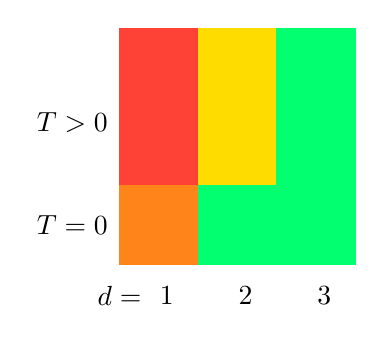
\begin{tikzpicture}
\node at (0,-0.4) {$d=$};
\node at (0.6,-0.4) {$1$};
\node at (1.6,-0.4) {$2$};
\node at (2.6,-0.4) {$3$};
\node at (-0.6,0.5) {$T=0$};
\node at (-0.6,1.8) {$T>0$};
\draw[draw=red1,fill=red1] (0,0) rectangle (1,3);
\draw[draw=orange1,fill=orange1] (0,0) rectangle (1,1);
\draw[draw=yellow1,fill=yellow1] (1,0) rectangle (2,3);
\draw[draw=green1,fill=green1] (1,0) rectangle (2,1);
\draw[draw=green1,fill=green1] (2,0) rectangle (3,3);
\end{tikzpicture}
\caption{Upper bounds for the decay of correlations. 
Red indicates exponential decay, yellow power law decay, and green ordered system.
Orange indicates exponential decay if the system is non-critical,
and power law if it is critical.}
\end{figure}

\begin{figure}
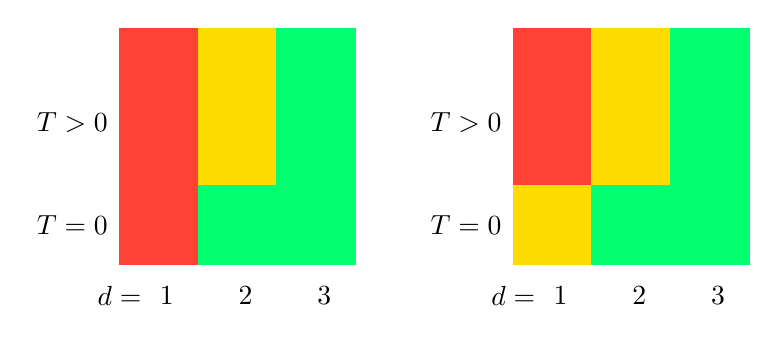
\begin{tikzpicture}
\node at (0,-0.4) {$d=$};
\node at (0.6,-0.4) {$1$};
\node at (1.6,-0.4) {$2$};
\node at (2.6,-0.4) {$3$};
\node at (-0.6,0.5) {$T=0$};
\node at (-0.6,1.8) {$T>0$};
\draw[draw=red1,fill=red1] (0,0) rectangle (1,3);
\draw[draw=yellow1,fill=yellow1] (1,0) rectangle (2,3);
\draw[draw=green1,fill=green1] (1,0) rectangle (2,1);
\draw[draw=green1,fill=green1] (2,0) rectangle (3,3);
%
\node at (5,-0.4) {$d=$};
\node at (5.6,-0.4) {$1$};
\node at (6.6,-0.4) {$2$};
\node at (7.6,-0.4) {$3$};
\node at (4.4,0.5) {$T=0$};
\node at (4.4,1.8) {$T>0$};
\draw[draw=red1,fill=red1] (5,0) rectangle (6,3);
\draw[draw=yellow1,fill=yellow1] (5,0) rectangle (6,1);
\draw[draw=yellow1,fill=yellow1] (6,0) rectangle (7,3);
\draw[draw=green1,fill=green1] (6,0) rectangle (7,1);
\draw[draw=green1,fill=green1] (7,0) rectangle (8,3);
\end{tikzpicture}
\caption{Upper bounds for the decay of correlations for (\emph{left}) a critical system,
and (\emph{right}) a non-critical system.
Red indicates exponential decay, yellow power law decay, and green ordered system.}
\end{figure}
\end{document}